%% Begin copyright
%%
%%  /home/jrf/Documents/books/Books20/Docs/Hjs/hjs_catalogue.tex
%%
%%   Part of the Books20 Project
%%
%%   Copyright 2022 James R. Fowler
%%
%%   All rights reserved. No part of this publication may be
%%   reproduced, stored in a retrival system, or transmitted
%%   in any form or by any means, electronic, mechanical,
%%   photocopying, recording, or otherwise, without prior written
%%   permission of the author.
%%
%%
%% End copyright
%
% History
% created 11 June 2022
%
%----------------------------------------------------------
\documentclass[letterpaper]{book}

\usepackage[T1]{fontenc}

\usepackage{graphicx}
\usepackage{wrapfig}
\usepackage[noautomatic]{imakeidx}
%\usepackage{imakeidx}
\usepackage[titlesize=12pt,parsize=10pt]{colophon}
\usepackage{books20}
\addglobalbib{../MasterBib.bib}
\addbibresource{hjs_baas_obit.bib}
\addbibresource{hjs.bib}

\newcommand*{\myhref}[1]{\hyperlink{entry:#1}{#1}}
\newcommand*{\bkfont}{\fontfamily{LibreCsln-TLF}\selectfont}
\DeclareTextFontCommand{\bookfont}{\bkfont}

\makeindex[name=author,title=Author/Editor Index]

\begin{document}

\frontmatter
\pagestyle{empty}
\title{\textsc{Catalogue of the \\
    Harlan J.\ Smith Collection \\
    of Science Books \\
    in the Otto Struve Library of \\
    the McDonald Observatory \\
    Fort Davis, Texas}}
\author{compiled by James R. Fowler}
\date{copy of \today}
\maketitle
\newpage
\vspace*{5 in}
\centerline{Copyright \copyright 2022 McDonald Observatory}
\centerline{Fort Davis, Texas}
\newpage

\pagestyle{plain}
\begin{figure}[t]
  \centering
  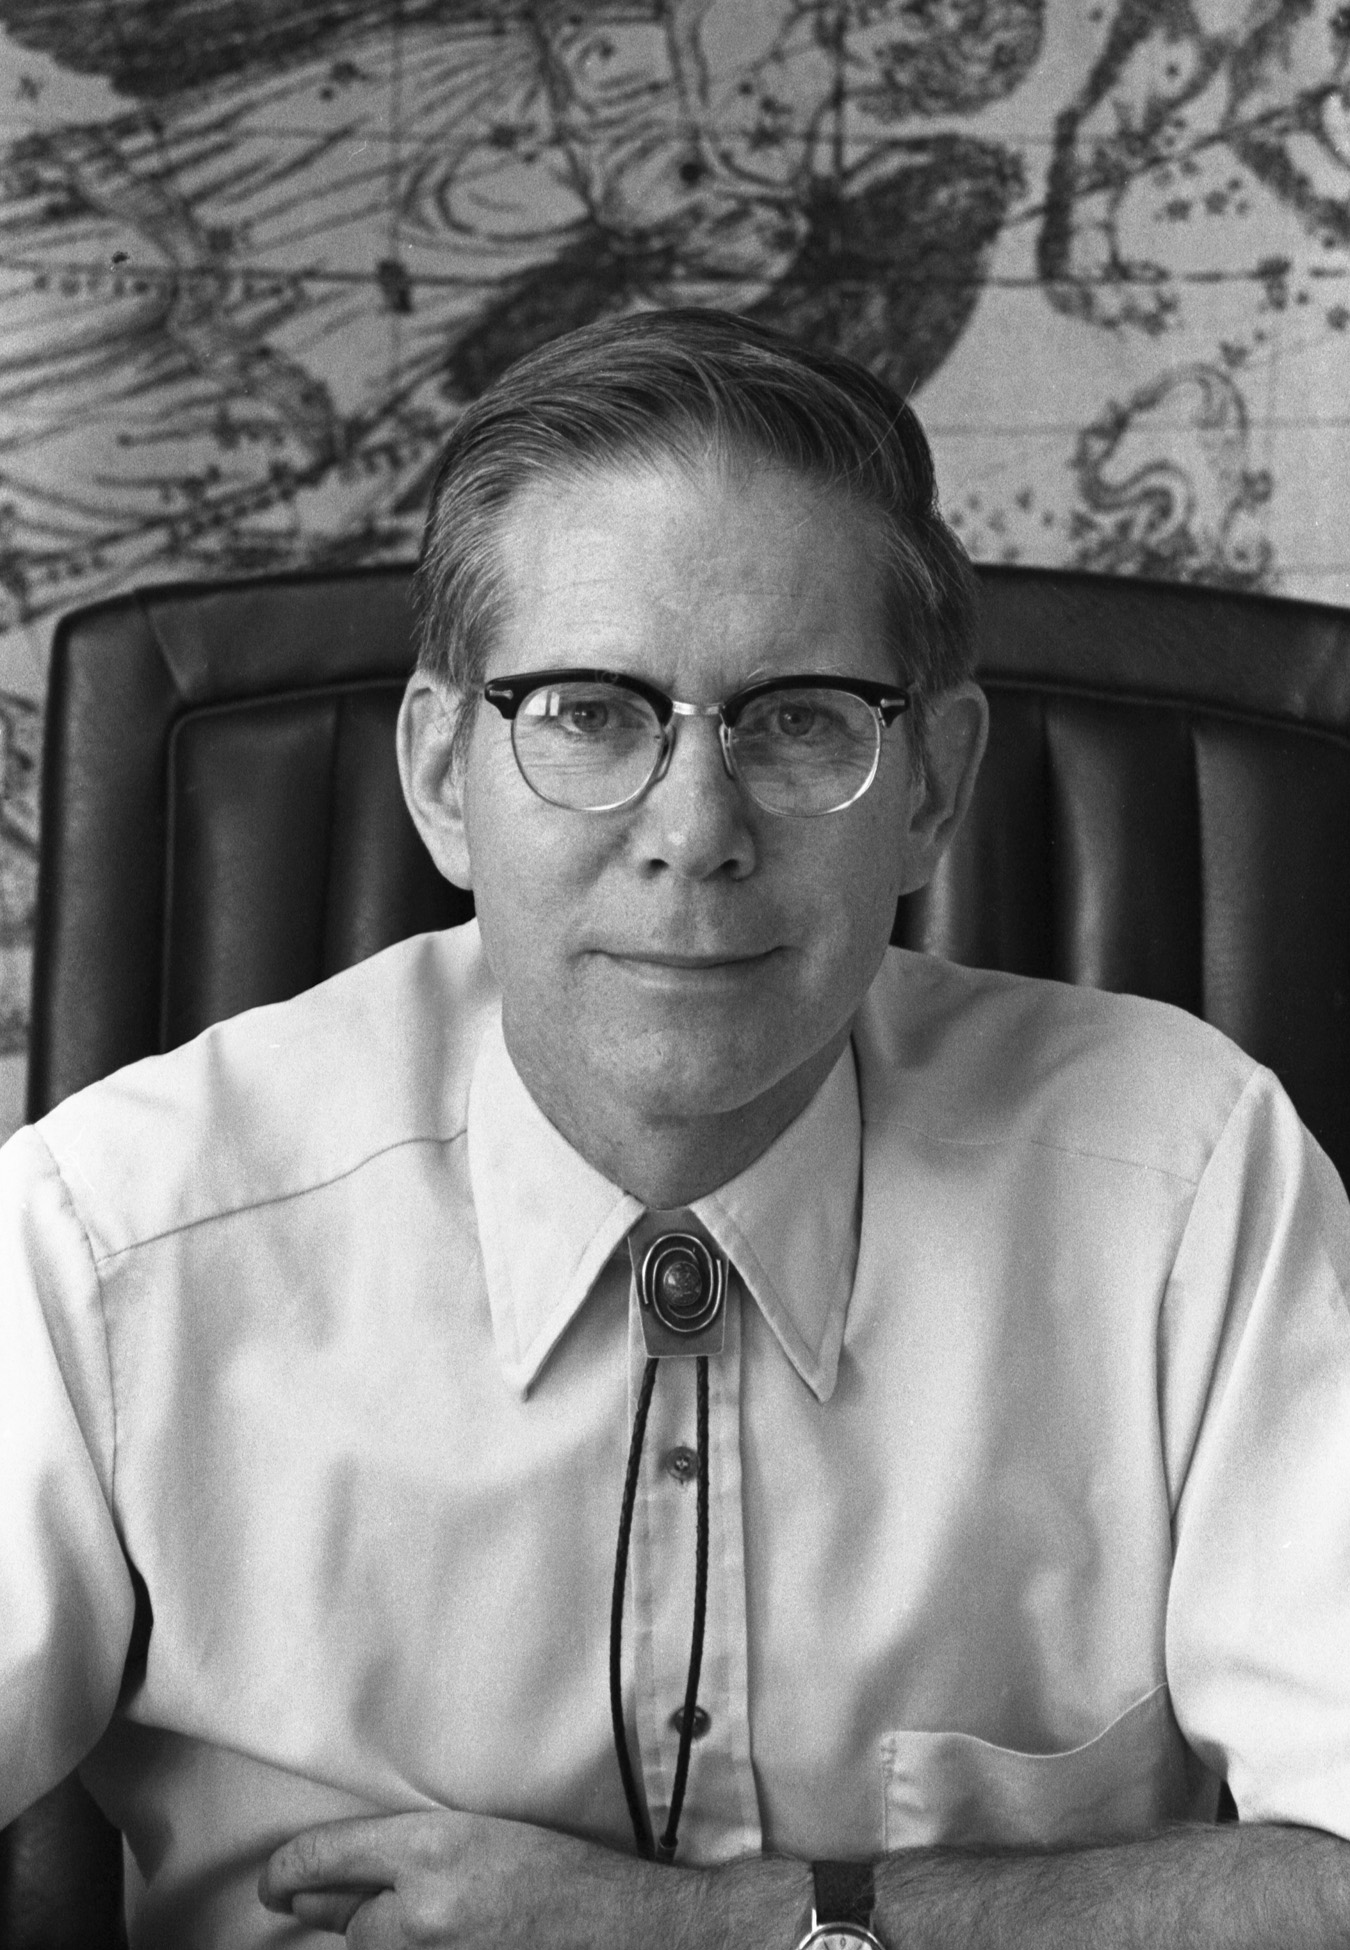
\includegraphics{hjs_photo.jpg}
  Harlan J.~Smith 1924 -- 1991 \\
  from Wikipedia
  (https://en.wikipedia.org/wiki/Harlan\_James\_Smith)
  \label{fig:hjs}
\end{figure}
\clearpage
\mbox{}
\thispagestyle{empty}
\newpage


\vspace*{1 in}
\centerline{\Large \bf Harlan J.\ Smith}
\bigskip\bigskip
\import{./}{biography}
\newpage

\vspace*{1 in}
\centerline{\Large \bf The Books}
\bigskip\bigskip
\import{./}{library}
\newpage
%%\showthe\font

\printbibliography

\mainmatter
\begin{center}
  {\Large \bf Catalogue of the Harlan J.\ Smith Collection}
\end{center}
\bigskip
\import{./}{books}

%%\showthe\font

\backmatter

\indexprologue{This index gives the page numbers where the particular author/editor(s) can be found.}
\printindex[author]

\begin{colophon}
  The catalogue was typeset with the \LaTeX2e\ processing system using
  10pt Computer Modern Roman font. The titles of the catalogue entries
  are in the Libre Caslon Bold font. This was printed and
  bound by J.~Fowler.
\end{colophon}

\end{document}

